\begin{figure}[h]
    \centering
    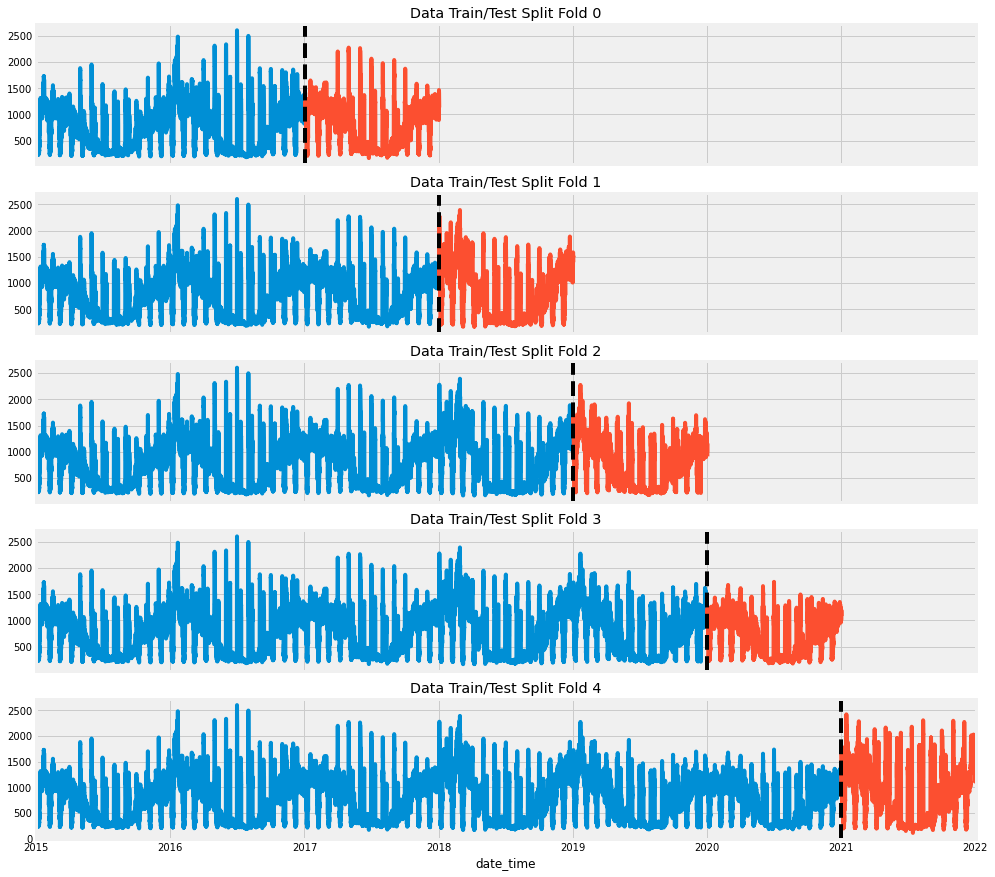
\includegraphics[width=15cm]{report/images/ts-cross-validation.png}
    \caption{Cross validation using Time Series Splits with each split being a year.}
    \label{fig:ts-cross-validation}
\end{figure}

\begin{figure}[h] 
\centering
\includegraphics[width=\textwidth]{}
\caption{A simplified diagram on how we assumed different components could affect each other and thus the target value.}
\label{fig:components} 
\end{figure}